%\bigbreak

\begin{figure}[!h]
\begin{adjustwidth}{-1.5cm}{}
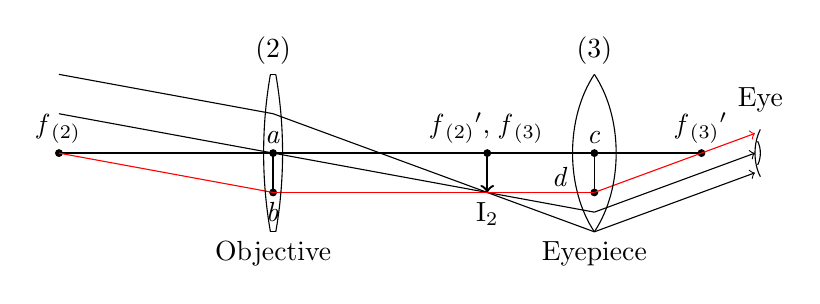
\begin{tikzpicture}[xscale = 0.68][yscale=2]
  \coordinate (x) at (0,0);
  \node at (x) {};
  \coordinate (y) at (12,0);
  \node at (y) {};
  \draw[line width=0.2mm] (x) -- (y);
  \coordinate (a) at (4,0);
  \node[above] at (a) {\textit{a}}; 
  \fill[shift only](a) circle [radius=.5mm];
  \coordinate (b) at (4,-0.5);
  \node[below] at (b) {\textit{b}}; 
  \fill[shift only](b) circle [radius=.5mm];
  \coordinate (c) at (10,0);
  \node[above] at (c) {\textit{c}};
  \fill[shift only](c) circle [radius=.5mm];
  \coordinate (d) at (10,-0.5);
  \node[above = 2mm, left = 2mm] at (d) {\textit{d}}; 
  \fill[shift only](d) circle [radius=.5mm];
  \draw[line width=0.2mm] (a) -- (b);
  \draw[line width=0.2mm] (c) -- (d);
  %--- Image
  \coordinate (ix) at (8,0);
  \coordinate (i) at (8,-0.5);
  \node[below] at (i) {I\textsubscript{2}};
  \node[above] at (ix) {\textit{f}\textsubscript{(2)}$'$, \textit{f}\textsubscript{(3)}};
  \fill[shift only](ix) circle [radius=.5mm];
  \draw[line width = 0.3mm, ->] (ix) -- (i);
  %--- Focal Points
  \coordinate (f1) at (0,0);
  \node[above] at (f1){\textit{f}\textsubscript{(2)}};
  \fill[shift only](f1) circle [radius=.5mm];
  \coordinate (f2) at (12,0);
  \node[above] at (f2){\textit{f}\textsubscript{(3)}$'$};
  \fill[shift only](f2) circle [radius=.5mm];
  %---Rays
  \draw[] (0,1) -- (4,0.5);
  \draw[] (0,0.5) -- (4,0);
  \draw[red] (x) -- (b);
  
  \draw[] (4,0.5) -- (10,-1);
  \draw[] (4,0) -- (10,-0.75);
  \draw[red] (4,-0.5) -- (10,-0.5);
  
  \draw[->] (10,-1) -- (13,-0.25);
  \draw[->] (10,-0.75) -- (13,-0);
  \draw[red, ->] (10,-0.5) -- (13,0.25);
  \coordinate (p) at (13.1,0);
  \node[above = 4mm] at (p){Eye};
  %\fill[shift only](p) circle [radius=1mm];
  \pgfmathsetmacro{\lensRadius}{0.5}
  \pgfmathsetmacro{\lensHeight}{0.3}
  \pgfmathsetmacro{\startAngle}{asin(\lensHeight/\lensRadius)}
  \draw (13.1,\lensHeight) arc[start angle=180-\startAngle,delta angle=2*\startAngle,radius=\lensRadius];
%  \draw (13,\lensHeight) arc[start angle=180-\startAngle,delta angle=2*\startAngle,radius=\lensRadius];
  \draw (13.05,0.15) arc[start angle=\startAngle,delta angle=-2*\startAngle,radius=\lensRadius/2];  
  %--- Lenses
  \pgfmathsetmacro{\lensRadius}{4}
  \pgfmathsetmacro{\lensHeight}{1}
  \pgfmathsetmacro{\startAngle}{asin(\lensHeight/\lensRadius)}
  \draw (3.95,\lensHeight) arc[start angle=180-\startAngle,delta angle=2*\startAngle,radius=\lensRadius];
  \draw (4.05,\lensHeight) arc[start angle=\startAngle,delta angle=-2*\startAngle,radius=\lensRadius];
  \draw[-] (3.95,1) -- (4.05,1);
  \draw[-] (3.95,-1) -- (4.05,-1);
  \node[below] at (4,-1){Objective};
  \node[above] at (4,1){(2)};
  \pgfmathsetmacro{\lensRadius}{1.43}
  \pgfmathsetmacro{\lensHeight}{1}
  \pgfmathsetmacro{\startAngle}{asin(\lensHeight/\lensRadius)}
  \draw (10,\lensHeight) arc[start angle=180-\startAngle,delta angle=2*\startAngle,radius=\lensRadius];
  \draw (10,\lensHeight) arc[start angle=\startAngle,delta angle=-2*\startAngle,radius=\lensRadius];
  \node[below] at (10,-1){Eyepiece};
  \node[above] at (10,1){(3)};
\end{tikzpicture}
\caption{Ray diagram}
\label{fig:ray}
\end{adjustwidth}
\end{figure}

